\documentclass[12pt]{beamer}

\usepackage{beamerthemeCambridgeUS}
\usepackage{textpos}
\usepackage{ragged2e}

\graphicspath{{G:/My Drive/FIGURAS/}}

\title[Principios de ocurrencia]{CARTOGRAFÍA GEOTÉCNICA}
\author[Edier Aristizábal]{Edier V. Aristizábal G.}
\institute{\emph{evaristizabalg@unal.edu.co}}
\date{Version:\today}

\addtobeamertemplate{headline}{}{%
	\begin{textblock*}{2mm}(.9\textwidth,0cm)
	\hfill
\includegraphics[height=1cm]{un}  
	\end{textblock*}}

\begin{document}
%%%%%%%%%%%%%%%%%%%%%%%%%%%%%%%%%%%%%%%%%%%%%%%%%%%%%%%%%%%%%%%%
\begin{frame}
\titlepage
\centering
\includegraphics[width=5cm]{unal}\hspace*{4.75cm}~%
\includegraphics[width=2cm]{logo3} 
\end{frame}
%%%%%%%%%%%%%%%%%%%%%%%%%%%%%%%%%%%%%%%%%%%%%%%%%%%%%%%%%%%%%%%%
\begin{frame}
\frametitle{Modelación}
\begin{figure}
\centering
\includegraphics[scale=0.40]{naturaleza} 
\end{figure}
\tiny{Fuente: Guzzetti (2015)}
\end{frame}
%%%%%%%%%%%%%%%%%%%%%%%%%%%%%%%%%%%%%%%%%%%%%%%%%%%%%%%%%%%%%%%%
\begin{frame}
\frametitle{Modelación}
\begin{figure}
\centering
\includegraphics[scale=0.40]{realidad-modelo} 
\end{figure}
\end{frame}
%%%%%%%%%%%%%%%%%%%%%%%%%%%%%%%%%%%%%%%%%%%%%%%%%%%%%%%%%%%%%%%%
\begin{frame}
\frametitle{Modelación}
\begin{figure}
\centering
\includegraphics[scale=0.4]{box} 
\end{figure}
\end{frame}
%%%%%%%%%%%%%%%%%%%%%%%%%%%%%%%%%%%%%%%%%%%%%%%%%%%%%%%%%%%%%%%%
\begin{frame}
\frametitle{Zonificación}
\scriptsize{
\textbf{Zonificación}: división del terreno en áreas homogéneas o dominios y su rango de acuerdo al grado actual o potencial de susceptibilidad, amenaza o riesgo por deslizamiento.
}
\begin{figure}
\centering
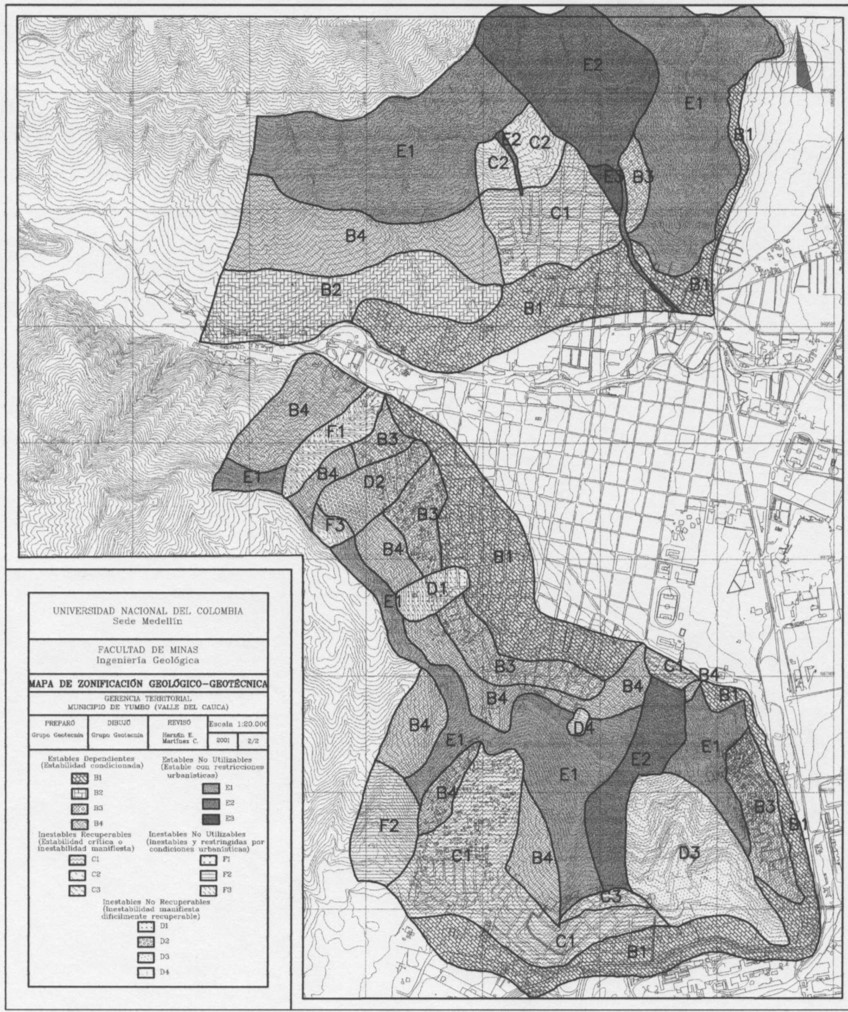
\includegraphics[scale=0.40]{zonificacion} 
\end{figure}
\end{frame}
%%%%%%%%%%%%%%%%%%%%%%%%%%%%%%%%%%%%%%%%%%%%%%%%%%%%%%%%%%%%%%%%
\begin{frame}
\frametitle{Susceptibilidad vs. Amenaza vs. Riesgo}
\scriptsize{
\begin{itemize}
\item \textbf{Mapas de incidencia espacial}\\
\textbf{Susceptibilidad}: tendencia de un movimiento en masa a ser generado en el futuro en un área específica (Brad, 1984). Posibilidad de que un fenómeno ocurra en un área de acuerdo con las condiciones locales del terreno, y especifican que factores detonantes tales como precipitación o sismicidad no son considerados (Soeters y van Westen, 1996).  Dónde: \emph{Probabilidad espacial}.
\item \textbf{Mapas de incidencia espacio-temporal y pronóstico}\\
\textbf{Amenaza}: probabilidad de ocurrencia de un potencial fenómeno destructivo dentro de un específico período de tiempo y en una determinada área (Varnes, 1984). Dónde (intensidad)? Cuándo (frecuencia), Magnitud (Volumen). \emph{Probabilidad espacial y temporal}.
\item \textbf{Mapas de evaluación de las consecuencias}\\
\textbf{Riesgo}: Evaluación de las potenciales consecuencias en términos de pérdidas humanas y pérdidas económicas. \textbf{Dónde}? (intensidad) \textbf{Cuándo}? (frecuencia) \textbf{Magnitud} (Volumen) \textbf{Cuánto}? (consecuencia)
\end{itemize}
}
\begin{figure}
\centering
\includegraphics[scale=0.6]{amenaza2} 
\end{figure}
\end{frame}
%%%%%%%%%%%%%%%%%%%%%%%%%%%%%%%%%%%%%%%%%%%%%%%%%%%%%%%%%%%%%%%%%%%%%
\begin{frame}
\frametitle{Zonificación}
\begin{figure}
\centering
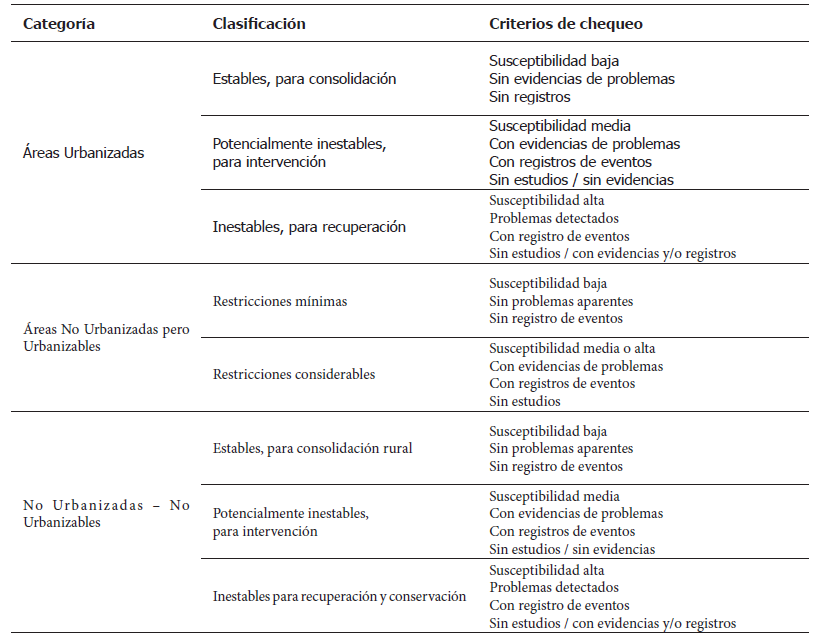
\includegraphics[scale=0.45]{zonificacion1} 
\end{figure}
\end{frame}
%%%%%%%%%%%%%%%%%%%%%%%%%%%%%%%%%%%%%%%%%%%%%%%%%%%%%%%%%%%%%%%%
\begin{frame}
\frametitle{Zonificación de la amenaza}
\scriptsize{
\textbf{Zonificación de amenaza}: La subdivisión del terreno en zonas que son caracterizadas por la probabilidad temporal de la ocurrencia de deslizamientos de un particular tamaño y forma, dentro de un periodo de tiempo dado. Los mapas de amenaza por deslizamientos deben indicar tanto la zona donde el deslizamiento puede ocurrir como la zona de propagación. Una completa evaluación de la amenaza por deslizamientos cuantitativa incluye:
\vfill
\begin{itemize}
\item \textbf{Probabilidad espacial}: la probabilidad que un área dada sea golpeada por un deslizamiento.
\vfill
\item \textbf{Probabilidad temporal}: la probabilidad que un evento detonante dado causará un deslizamiento.
\vfill
\item \textbf{Probabilidad de tamaño/volumen}: probabilidad que un deslizamiento tenga un determinado tamaño y volumen.
\vfill
\item \textbf{Probabilidad de propagación}: probabilidad que un deslizamiento alcanzará una cierta distancia ladera abajo.
\end{itemize}
}
\vfill
\tiny{Fuente: AGS (2007), Corominas et al. (2014)}
\end{frame}
%%%%%%%%%%%%%%%%%%%%%%%%%%%%%%%%%%%%%%%%%%%%%%%%%%%%%%%%%%%%%%%%%%%%%
\begin{frame}
\frametitle{Hipótesis}
\scriptsize{
Varnes (1984) y Guzzetti (2006) definen  algunos principios básicos o hipótesis para la zonificación:
\vfill
\begin{itemize}
\item El pasado es la clave del presente, lo que implica que los deslizamientos en el futuro ocurrirán bajo las condiciones que se generaron en el pasado.
\vfill
\item Los deslizamientos dejan característica identificables que pueden ser reconocidas, clasificadas y mapeadas en el campo o a través de sensores remotos. Por qué el movimiento en masa ocurrió, cuándo y dónde ocurrió, y los mecanismos?
\vfill
\item Los deslizamientos están controlados por leyes mecánicas que pueden ser determinadas empíricamente, estadísticamente o deterministicamente. 
\vfill
\item Las condiciones que causan los deslizamientos, directa e indirectamente están relacionadas con los deslizamientos, pueden ser recolectadas y utilizadas para modelos de predicción de la ocurrencia de deslizamientos.
\vfill
\item La ocurrencia de deslizamientos, en tiempo y espacio, puede ser inferido desde investigación heurísticas utilizando el análisis de la información ambiental o inferida de modelos físicos. Por lo que un territorio puede ser zonificado entre zonas de susceptibilidad o amenaza graduadas de acuerdo con las diferentes probabilidades.
\end{itemize}
}
\end{frame}
%%%%%%%%%%%%%%%%%%%%%%%%%%%%%%%%%%%%%%%%%%%%%%%%%%%%%%%%%%%%%%%%%%%%%
\begin{frame}
\frametitle{Escala}
\begin{figure}
\centering
\includegraphics[scale=0.5]{escala-zonificacion} 
\end{figure}
\tiny{Fuente: Fell et al (2008) del JTC-1 Technical Committee on Landslides and Engineered Slopes}
\end{frame}
%%%%%%%%%%%%%%%%%%%%%%%%%%%%%%%%%%%%%%%%%%%%%%%%%%%%%%%%%%%%%%%%
\begin{frame}
\frametitle{Escala y Fases}
\begin{figure}
\centering
\includegraphics[scale=0.5]{fases} 
\end{figure}
\end{frame}
%%%%%%%%%%%%%%%%%%%%%%%%%%%%%%%%%%%%%%%%%%%%%%%%%%%%%%%%%%%%%%%%
\begin{frame}
\frametitle{Escala de sitio: Geotecnia}
\framesubtitle{Fase de diseño de obras de ingeniería}
\begin{figure}
\centering
\includegraphics[scale=0.5]{escala-sitio} 
\end{figure}
\end{frame}
%%%%%%%%%%%%%%%%%%%%%%%%%%%%%%%%%%%%%%%%%%%%%%%%%%%%%%%%%%%%%%%%
\begin{frame}
\frametitle{Zonificación: Cartografía Geotécnica}
\framesubtitle{Ordenar el territorio}
\begin{figure}
\centering
\includegraphics[scale=0.5]{zonificacion-detalle} 
\end{figure}
\end{frame}
%%%%%%%%%%%%%%%%%%%%%%%%%%%%%%%%%%%%%%%%%%%%%%%%%%%%%%%%%%%%%%%%
\begin{frame}
\frametitle{Zonificación: Cartografía Geotécnica}
\framesubtitle{Regional}
\begin{figure}
\centering
\includegraphics[scale=0.5]{zonificacion-media} 
\end{figure}
\end{frame}
%%%%%%%%%%%%%%%%%%%%%%%%%%%%%%%%%%%%%%%%%%%%%%%%%%%%%%%%%%%%%%%%
\begin{frame}
\frametitle{Zonificación: Cartografía Geotécnica}
\framesubtitle{Regional - cuenca}
\begin{figure}
\centering
\includegraphics[scale=0.47]{zonificacion-cuenca} 
\end{figure}
\end{frame}
%%%%%%%%%%%%%%%%%%%%%%%%%%%%%%%%%%%%%%%%%%%%%%%%%%%%%%%%%%%%%%%%
\begin{frame}
\frametitle{Zonificación: Cartografía Geotécnica}
\framesubtitle{Escala nacional}
\begin{figure}
\centering
\includegraphics[scale=0.5]{zonificacion-nacional} 
\end{figure}
\end{frame}
%%%%%%%%%%%%%%%%%%%%%%%%%%%%%%%%%%%%%%%%%%%%%%%%%%%%%%%%%%%%%%%%
\begin{frame}
\frametitle{Metodología}
\scriptsize{
\begin{itemize}
\item Formulación del problema y definición de alcances
\vfill
\item Levantamiento de datos: 
\vfill
\item La identificación y mapeo de eventos en el área de estudio (variable dependiente),
\vfill
\item La identificación y mapeo de los factores físicos que están directa o indirectamente correlacionados con los factores de inestabilidad (variables predictoras e independientes),
\vfill
\item Análisis exploratorio de datos y selección de variables,
\vfill
\item Construcción del modelo,
\vfill
\item La clasificación del terreno en dominios  de diferentes niveles de susceptibilidad,
\vfill
\item La evaluación del desempeño y capacidad de predicción del modelo,
\vfill
\item Validación y ajuste heurístico en campo.
\end{itemize}
}
\vfill
\tiny{Fuente: Guzzetti (2006) Landslide susceptibility zoning }
\end{frame}
%%%%%%%%%%%%%%%%%%%%%%%%%%%%%%%%%%%%%%%%%%%%%%%%%%%%%%%%%%%%%%%%%%%
\begin{frame}
\frametitle{Herramientas}
\scriptsize{
\begin{itemize}
\item \textbf{Vector GIS}: para mapear los deslizamientos y generar los mapas temáticos de salida, ArcGIS, SPRING, QGIS etc,.
\vfill
\item \textbf{Raster GIS}: para procesamiento de imágenes de satélite, y para el procesamiento de los factores condicionantes a partir del MDT: Erdas Imagine, ArcGIS.
\vfill
\item \textbf{Paquetes estadísticos}: para test estadísticos y análisis multivariados, como regresión logística o análisis discriminado: SPSS, R, etc.
\vfill
\item \textbf{Otros}: compiladores de programación para diseñar códigos específicos y procesar datos o análisis, tales como Python, JS, Matlab, etc.
\end{itemize}
}
\end{frame}
%%%%%%%%%%%%%%%%%%%%%%%%%%%%%%%%%%%%%%%%%%%%%%%%%%%%%%%%%%%%%%%%%%%
\begin{frame}
\frametitle{Definición área de influencia}
\scriptsize{
\textbf{Unidades Morfodinámicas Independientes (UMI) }son definidas como la unidad del territorio que enmarca la ladera de interés y que presenta un comportamiento independiente de las unidades adyacentes (Chica, 1989). Se considera que cualquier proceso morfodinámico que se presente en el exterior no afecta su interior e igualmente, cualquier proceso morfodinámico que se presente en el interior no afecta las unidades adyacentes (AMVA et al., 2012). Dicha unidad es delimitada por divisorias de agua, drenajes o expresiones geomorfológicas, combinadas con un análisis heurístico de la morfodinámica del paisaje. 
}
\begin{figure}
\centering
\includegraphics[scale=0.3]{area-influencia} 
\end{figure}
\end{frame}
%%%%%%%%%%%%%%%%%%%%%%%%%%%%%%%%%%%%%%%%%%%%%%%%%%%%%%%%%%%%%%%%
\begin{frame}
\frametitle{Unidad de análisis}
\framesubtitle{\emph{Terrain Mapping Unit -TMU-}}
\scriptsize{
La unidad de mapeo representa el dominio que maximiza la homogeneidad interna y la heterogeneidad entre unidades. Se refiere a la porción del territorio que contiene un grupo de condiciones del terreno que difiere de la unidad adyacente a lo largo de limites definidos (Hansen, 1984).
 
}
\begin{figure}
\centering
\includegraphics[scale=0.45]{unidad-analisis} 
\end{figure}
\tiny{Tomado de Berry – Map Analysis}
\end{frame}
%%%%%%%%%%%%%%%%%%%%%%%%%%%%%%%%%%%%%%%%%%%%%%%%%%%%%%%%%%%%%%%%
\begin{frame}
\frametitle{Unidad de análisis}
\framesubtitle{Malla de celdas\emph{(Grid-cells)}}
\scriptsize{
Dividen el territorio en rectángulos regulares, triangulares, hexagonales, etc, de tamaño predefinido. Son preferidos por usuarios GIS basados en raster. Cada celda es asignada con un valor para cada factor morfométrico, geológico, usos del suelo, etc. 
}
\begin{figure}
\centering
\includegraphics[scale=0.45]{tmu1} 
\end{figure}
\scriptsize{\textbf{Desventajas}: No representan un significado físico para el territorio.}
\vfill
\tiny{Fuente: Guzzetti (2005)}
\end{frame}
%%%%%%%%%%%%%%%%%%%%%%%%%%%%%%%%%%%%%%%%%%%%%%%%%%%%%%%%%%%%%%%%
\begin{frame}
\frametitle{Unidad de análisis}
\framesubtitle{Unidad de ladera\emph{(slope-units)}}
\scriptsize{
Automáticamente derivado de DTM de alta calidad, partiendo el territorio en regiones hidrológicas entre drenajes y líneas de división de cuencas, es decir subcuentas de acuerdo a la escala de análisis.
}
\begin{figure}
\centering
\includegraphics[scale=0.45]{tmu2} 
\end{figure}
\scriptsize{\textbf{Desventajas}: Dificultad en la preparación, y pueden no corresponder a subdivisiones importantes para determinar la susceptibilidad a deslizamientos.}
\vfill
\tiny{Fuente: Guzzetti (2005)}
\end{frame}
%%%%%%%%%%%%%%%%%%%%%%%%%%%%%%%%%%%%%%%%%%%%%%%%%%%%%%%%%%%%%%%%
\begin{frame}
\frametitle{Unidad de análisis}
\framesubtitle{Unidad de de Condiciones Unicas (UCU)}
\scriptsize{
Son dominios homogéneos derivados desde una clasificación de muchos factores de estabilidad de laderas.
}
\begin{figure}
\centering
\includegraphics[scale=0.4]{tmu3} 
\end{figure}
\scriptsize{\textbf{Desventajas}: Pueden generarse muchos pequeños polígonos difíciles de interpretar o manejar.
}
\vfill
\tiny{Fuente: Guzzetti (2005)}
\end{frame}
%%%%%%%%%%%%%%%%%%%%%%%%%%%%%%%%%%%%%%%%%%%%%%%%%%%%%%%%%%%%%%%%
\begin{frame}
\begin{figure}
\centering
\includegraphics[scale=0.5]{unidad-analisis1} 
\end{figure}
\tiny{Fuente: Guzzetti (2006) Landslide susceptibility zoning }
\end{frame}
%%%%%%%%%%%%%%%%%%%%%%%%%%%%%%%%%%%%%%%%%%%%%%%%%%%%%%%%%%%%%%%%
\begin{frame}
\begin{figure}
\centering
\includegraphics[scale=0.5]{slope-units} 
\end{figure}
\end{frame}
%%%%%%%%%%%%%%%%%%%%%%%%%%%%%%%%%%%%%%%%%%%%%%%%%%%%%%%%%%%%%%%%
\begin{frame}
\frametitle{Métodos de zonificación}
\begin{figure}
\centering
\includegraphics[scale=0.5]{metodologias_menm} 
\end{figure}
\tiny{Modificado de AGS (2007) Guidelines for landslide susceptibility, hazard and risk assessment}
\end{frame}
%%%%%%%%%%%%%%%%%%%%%%%%%%%%%%%%%%%%%%%%%%%%%%%%%%%%%%%%%%%%%%%%
\begin{frame}
\frametitle{Métodos de zonificación}
\begin{figure}
\centering
\includegraphics[scale=0.5]{tabla-metodologias} 
\end{figure}
\tiny{Fuente: Guzzetti (2006) Landslide susceptibility zoning}
\end{frame}
%%%%%%%%%%%%%%%%%%%%%%%%%%%%%%%%%%%%%%%%%%%%%%%%%%%%%%%%%%%%%%%%
\begin{frame}
\frametitle{Métodos de zonificación}
\framesubtitle{Amenaza Relativa vs Absoluta}
\begin{figure}
\centering
\includegraphics[scale=0.5]{relativa-absoluta} 
\end{figure}
\tiny{Fuente: Hartlen \& Viberg (1988)}
\end{frame}
%%%%%%%%%%%%%%%%%%%%%%%%%%%%%%%%%%%%%%%%%%%%%%%%%%%%%%%%%%%%%%%%
\begin{frame}
\frametitle{Métodos de zonificación}
\begin{figure}
\centering
\includegraphics[scale=0.4]{metodologia-menm} 
\end{figure}
\tiny{Fuente: Aleotti \& Chowdhyry (1998) }
\end{frame}
%%%%%%%%%%%%%%%%%%%%%%%%%%%%%%%%%%%%%%%%%%%%%%%%%%%%%%%%%%%%%%%%
\begin{frame}
\frametitle{Zonificación}
\begin{figure}
\centering
\includegraphics[scale=0.5]{susceptibilidad-clasificacion} 
\end{figure}
\end{frame}
%%%%%%%%%%%%%%%%%%%%%%%%%%%%%%%%%%%%%%%%%%%%%%%%%%%%%%%%%%%%%%%%
\begin{frame}
\frametitle{Métodos de zonificación}
\begin{figure}
\centering
\includegraphics[scale=0.5]{metodologias-ml} 
\end{figure}
\end{frame}
%%%%%%%%%%%%%%%%%%%%%%%%%%%%%%%%%%%%%%%%%%%%%%%%%%%%%%%%%%%%%%%%
\begin{frame}
\frametitle{Métodos de zonificación}
\begin{figure}
\centering
\includegraphics[scale=0.5]{metodologias-tabla} 
\end{figure}
\tiny{Fuente: Huabin et al. (2005)}
\end{frame}
%%%%%%%%%%%%%%%%%%%%%%%%%%%%%%%%%%%%%%%%%%%%%%%%%%%%%%%%%%%%%%%%
\end{document}